\documentclass{beamer}

\mode<presentation> {

%\usetheme{default}
%\usetheme{AnnArbor}
%\usetheme{Antibes}
%\usetheme{Bergen}
%\usetheme{Berkeley}
%\usetheme{Berlin}
%\usetheme{Boadilla}
\usetheme{CambridgeUS}
%\usetheme{Copenhagen}
%\usetheme{Darmstadt}
%\usetheme{Dresden}
%\usetheme{Frankfurt}
%\usetheme{Goettingen}
%\usetheme{Hannover}
%\usetheme{Ilmenau}
%\usetheme{JuanLesPins}
%\usetheme{Luebeck}
%\usetheme{Madrid}
%\usetheme{Malmoe}
%\usetheme{Marburg}
%\usetheme{Montpellier}
%\usetheme{PaloAlto}
%\usetheme{Pittsburgh}
%\usetheme{Rochester}
%\usetheme{Singapore}
%\usetheme{Szeged}
%\usetheme{Warsaw}

% As well as themes, the Beamer class has a number of color themes
% for any slide theme. Uncomment each of these in turn to see how it
% changes the colors of your current slide theme.

%\usecolortheme{albatross}
%\usecolortheme{beaver}
%\usecolortheme{beetle}
%\usecolortheme{crane}
%\usecolortheme{dolphin}
%\usecolortheme{dove}
%\usecolortheme{fly}
%\usecolortheme{lily}
%\usecolortheme{orchid}
%\usecolortheme{rose}
%\usecolortheme{seagull}
%\usecolortheme{seahorse}
%\usecolortheme{whale}
%\usecolortheme{wolverine}

%\setbeamertemplate{footline} % To remove the footer line in all slides uncomment this line
%\setbeamertemplate{footline}[page number] % To replace the footer line in all slides with a simple slide count uncomment this line

%\setbeamertemplate{navigation symbols}{} % To remove the navigation symbols from the bottom of all slides uncomment this line
}

\usepackage{graphicx} % Allows including images
\usepackage{booktabs} % Allows the use of \toprule, \midrule and \bottomrule in tables
\usepackage{tikz}
\usepackage{pgfgantt}
\usetikzlibrary{shapes.geometric, arrows}
\tikzstyle{startstop} = [rectangle, rounded corners, minimum width=4cm, minimum height=1.3cm,text centered, draw=black, fill=red!30]
\tikzstyle{process} = [rectangle, minimum width=4cm, minimum height=1.3cm, text centered, draw=black, fill=orange!30]
\tikzstyle{decision} = [diamond, minimum width=4cm, minimum height=1.3cm, text centered, draw=black, fill=green!30]
\tikzstyle{arrow} = [thick,->,>=stealth]

\tikzstyle{dfdprocess} = [circle,draw=black, inner sep=0pt,minimum size=3cm, fill=red!30, text width=3cm, text centered]
\tikzstyle{dfdentity} = [rectangle, rounded corners, minimum width=3cm, minimum height=1.2cm,text centered, draw=black, fill=red!30]
\tikzset{data store/.style={
        minimum width=4.5cm,
        minimum height=1.2cm,
        append after command={
            \pgfextra
            \fill[fill=red!30] (\tikzlastnode.south east) [rounded corners] -| (\tikzlastnode.west) |- (\tikzlastnode.north) [sharp corners] -| (\tikzlastnode.north east)--cycle;
            \draw[rounded corners] (\tikzlastnode.south east) -| (\tikzlastnode.west) |- (\tikzlastnode.north east);
        \endpgfextra}
    }
}

\ganttset{group/.append style={orange},
milestone/.append style={red},
progress label node anchor/.append style={text=red}}
%----------------------------------------------------------------------------------------
%	TITLE PAGE
%----------------------------------------------------------------------------------------

\title[Automated Answer Paper Evaluation]{Automated Answer Paper Evaluation using Deep Learning \& NLP} % The short title appears at the bottom of every slide, the full title is only on the title page
\author{Team No. 16} % Your name
\vspace{-0.5cm}
\institute[Dept. of CSE, GCEK] % Your institution as it will appear on the bottom of every slide, may be shorthand to save space
{
% Roll. No.  \\S7 CSE (2016 Batch)\\ % Your institution for the title page
\begin{table}
    \centering
    \begin{tabular}{c c}
        \toprule
        \textbf{Name} & \textbf{Roll number}\\
        \midrule
        Pranav T N & 46\\
        Rahul Mohanan A K & 47\\
        Sourabh Subhod & 53\\
        Vishal V & 59\\
        \bottomrule
    \end{tabular}
\end{table}
S7 CSE (2016 Batch)\\
\textit{Guide: Prof. Sajith B}
% \textit{email@id.com} % Your email address
}
\date{\today} % Date, can be changed to a custom date
\begin{document}

\begin{frame}
\titlepage % Print the title page as the first slide
\end{frame}

\begin{frame}
\frametitle{Outline} % Table of contents slide, comment this block out to remove it
\tableofcontents % Throughout your presentation, if you choose to use \section{} and \subsection{} commands, these will automatically be printed on this slide as an overview of your presentation
\end{frame}

%	PRESENTATION SLIDES
%------------------------------------------------
\section{Project Objectives} 

%\subsection{} % A subsection can be created just before a set of slides with a common theme to further break down your presentation into chunks
\begin{frame}
\frametitle{Project Objectives}
\begin{itemize}
    \item Manual evaluation time consuming.
    \item Automated system preferred for fast evaluation.
    \item A handwriting recognition system based on a RNN architecture used for digital conversion of answer paper.
    \item A NLP model used for semantic evaluation of digital answer paper using provided answer key.
\end{itemize}
\end{frame}
\section{System Architecture}
% \subsection{Use Case Diagram}
\begin{frame}
    \frametitle{System Architecture}
    \begin{figure}[!h]
        \centering
        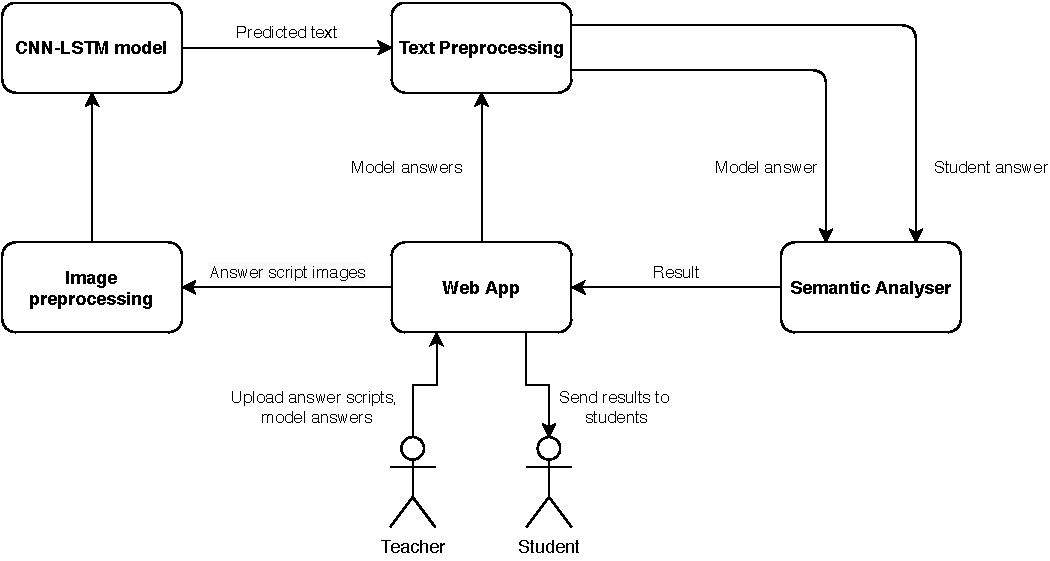
\includegraphics[scale=0.6]{images/arch.pdf}
        % \caption{}
        % \label{}
    \end{figure}
\end{frame}


\subsection{Handwritten Text Recognition Module}
\begin{frame}
    \frametitle{HTR Model}
    \begin{figure}[!h]
        \centering
        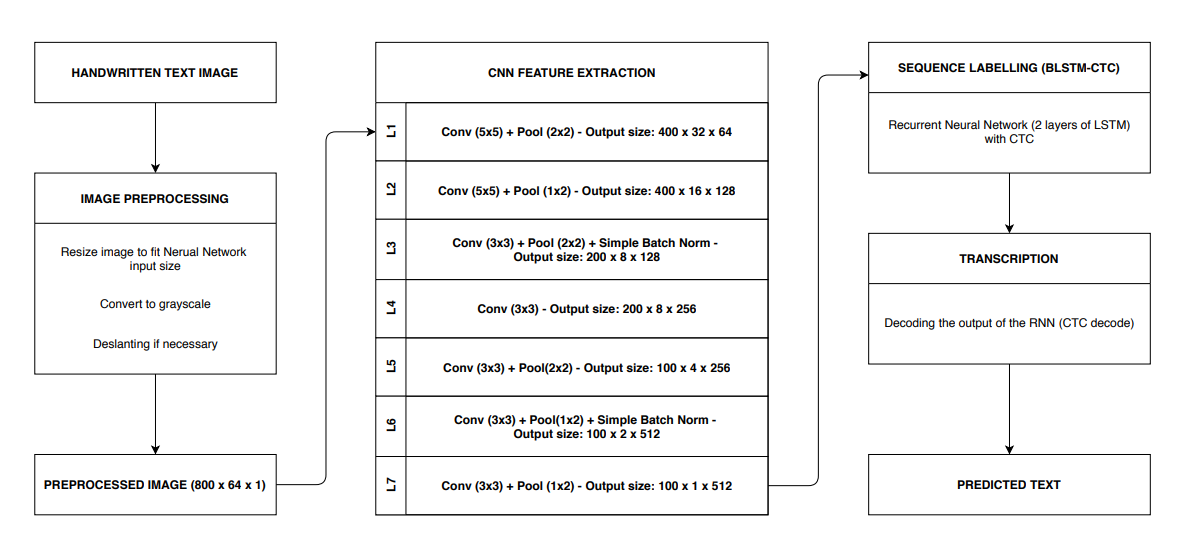
\includegraphics[scale=0.35]{images/htr.png}
        % \caption{}
        % \label{}
    \end{figure}
\end{frame}


\subsection{Classifier Architecture}
\begin{frame}
    \frametitle{Classifier Architecture}
    \begin{figure}[!h]
        \centering
        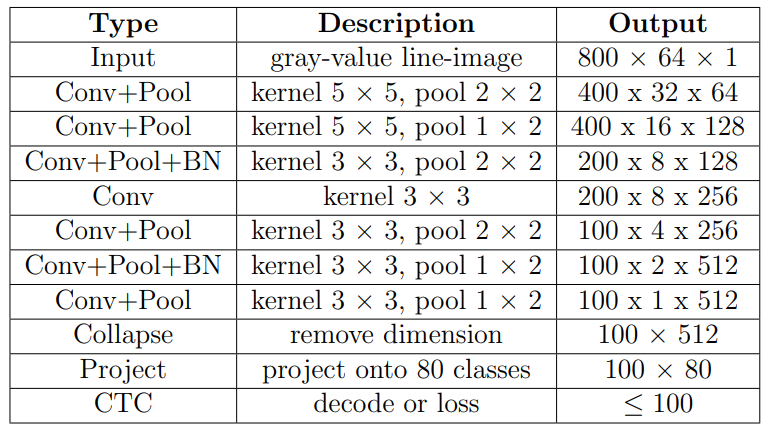
\includegraphics[scale=0.6]{images/clas.png}
        % \caption{}
        % \label{}
    \end{figure}
\end{frame}
\section{Non-Functional Requirements}
\begin{frame}
\frametitle{Non-Functional Requirements}
\begin{itemize}
    \item The system shall be able to perform evaluation with
    reasonable performance compared to manual evaluation.
    \item The system shall be accurate in recognizing handwriting
    from the answer papers.
    \item Apart from the initial cost, the system shall be less
    costly to maintain.
    \item The system shall be open-source.
    \item The system shall be usable on any platform.
\end{itemize}
\end{frame}
\section{Project Preliminary Design}

\subsection{Flow Charts}
\begin{frame}
    \frametitle{Flow Charts}
    \begin{figure}[!h]
        \centering
        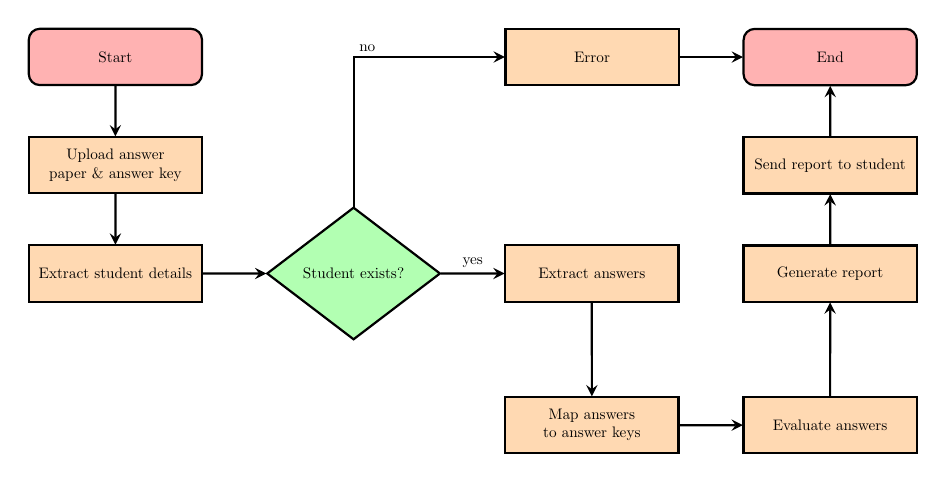
\begin{tikzpicture}[node distance=2.5cm,thick,scale=0.55, every node/.style={scale=0.55}]
            \node (start) [startstop] {Start};
            \node (pro1) [process, below of=start, text width=\textwidth-8.5cm] {Upload answer paper \& answer key};
            \node (pro2) [process, below of=pro1] {Extract student details};
            \node (dec1) [decision, right of=pro2, xshift=3cm] {Student exists?};
            \node (pro3) [process, right of=dec1, xshift=3cm] {Extract answers};
            \node (pro4) [process, text width=\textwidth-8.5cm, below of=pro3, yshift=-1cm] {Map answers to answer keys};
            \node (pro5) [process, right of=pro4, xshift=3cm] {Evaluate answers};
            \node (pro6) [process, above of=pro5, yshift=1cm] {Generate report};
            \node (pro7) [process, above of=pro6] {Send report to student};
            \node (end) [startstop, above of=pro7] {End};
            \node (error) [process, left of=end, xshift=-3cm] {Error};

            \draw [arrow] (start) -- (pro1);
            \draw [arrow] (pro1) -- (pro2);
            \draw [arrow] (pro2) -- (dec1);
            \draw [arrow] (dec1) -- node[anchor=south] {yes} (pro3);
            \draw [arrow] (dec1) |- node[anchor=south west] {no} (error);
            \draw [arrow] (pro3) -- (pro4);
            \draw [arrow] (pro4) -- (pro5);
            \draw [arrow] (pro5) -- (pro6);
            \draw [arrow] (pro6) -- (pro7);
            \draw [arrow] (pro7) -- (end);
            \draw [arrow] (error) -- (end);
        \end{tikzpicture}
        % \caption{}
        % \label{}
    \end{figure}
\end{frame}

\subsection{Data Flow Diagram - Level 0}

\begin{frame}
    \frametitle{Data Flow Diagram - Level 0}
        \begin{figure}[!h]
            \centering
            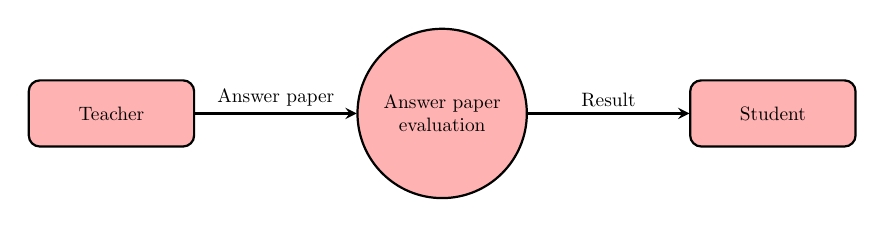
\begin{tikzpicture}[node distance=3cm,thick,scale=0.7, every node/.style={scale=0.7}]
                \node (proc1) [dfdprocess] {Answer paper evaluation};
                \node (teacher) [dfdentity, left of=proc1, xshift=-3cm] {Teacher};
                \node (student) [dfdentity, right of=proc1, xshift=3cm] {Student};

                \draw [arrow] (teacher) -- node[anchor=south] {Answer paper} (proc1);
                \draw [arrow] (proc1) -- node[anchor=south] {Result} (student);
            \end{tikzpicture}
            % \caption{}
            % \label{}
        \end{figure}
\end{frame}

\subsection{Data Flow Diagram - Level 1}

\begin{frame}
    \frametitle{Data Flow Diagram - Level 1}
        \begin{figure}[!h]
            \centering
            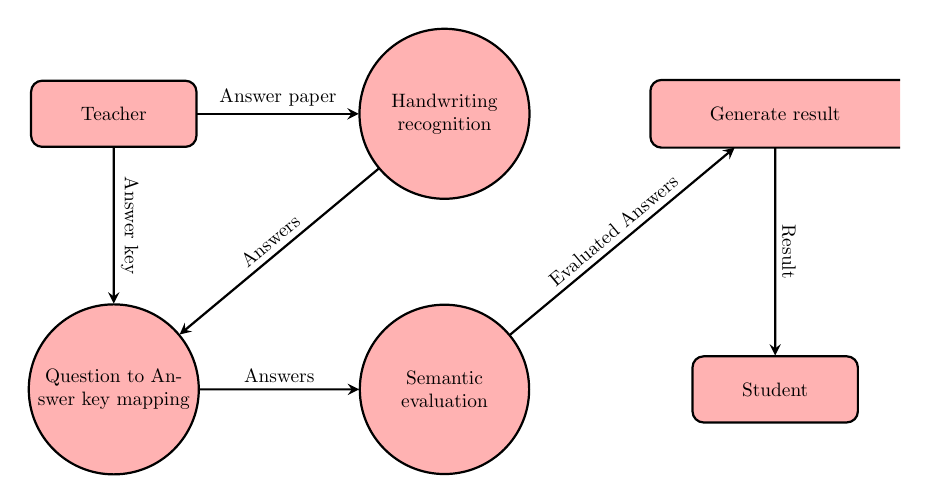
\begin{tikzpicture}[node distance=3cm,thick,scale=0.7, every node/.style={scale=0.7}]
                \node (proc1) [dfdprocess] {Handwriting recognition};
                \node (teacher) [dfdentity, left of=proc1, xshift=-3cm] {Teacher};
                \node (proc2) [dfdprocess, below of=teacher, yshift=-2cm] {Question to Answer key mapping};
                \node (proc3) [dfdprocess, right of=proc2, xshift=3cm] {Semantic evaluation};
                \node (result) [data store, right of=proc1, xshift=3cm] {Generate result};
                \node (student) [dfdentity, right of=proc3, xshift=3cm] {Student};

                \draw [arrow] (teacher) -- node[anchor=south] {Answer paper} (proc1);
                \draw [arrow] (teacher) -- node[rotate=-90, anchor=south] {Answer key} (proc2);
                \draw[arrow] (proc1) -- node[rotate=40, anchor=south] {Answers} (proc2);
                \draw[arrow] (proc2) -- node[anchor=south] {Answers} (proc3);
                \draw[arrow] (proc3) -- node[rotate=40,anchor=south] {Evaluated Answers} (result);
                \draw[arrow] (result) -- node[rotate=-90, anchor=south] {Result} (student);
            \end{tikzpicture}
            % \caption{}
            % \label{}
        \end{figure}
\end{frame}
\section{Work Plan - Gantt Chart}
\begin{frame}
    \frametitle{Work Plan - Gantt Chart}
    \noindent\resizebox{\textwidth}{!}{

    \begin{ganttchart}[%Specs
        x unit = 2cm,  %<---------------------- New x unit 
        y unit title=0.8cm,
        y unit chart=1cm,
        vgrid, hgrid,
        title height=1,
    %     title/.style={fill=none},
        title label font=\bfseries\footnotesize,
        bar/.style={fill=green},
        bar height=0.5,
        bar left shift=0.05,
        bar right shift=-0.05,
        progress label text={},
        group right shift=0,
        group top shift=0.7,
        group height=.3,
        group peaks width={0.2},
        inline]{1}{7}
       %labels
    
       \gantttitle{2019}{3}
       \gantttitle{2020}{4} \\                 % title 
       \gantttitle{October}{1}                      % title 3
       \gantttitle{November}{1}
       \gantttitle{December}{1}
       \gantttitle{January}{1}
       \gantttitle{February}{1}
       \gantttitle{March}{1}
       \gantttitle{April}{1}\\
    
       % Setting group if any
    
    %    \ganttgroup[inline=false]{Group 1}{1}{5}\\ 
    
       \ganttbar[inline=false]{Literature Survey}{1}{2}\\
       \ganttbar[progress=0,inline=false]{Create and train RNN model}{3}{4}\\       
       \ganttbar[progress=0,inline=false]{Separate answers and map to answer key}{4}{4}\\
       \ganttbar[progress=0,inline=false]{Create NLP Model}{4}{5}\\
       \ganttbar[progress=0,inline=false]{Test Primary System}{6}{6}\\
       \ganttbar[progress=0,inline=false]{Evaluation of performance}{7}{7}
    %    \ganttmilestone[inline=false]{Milestone 1}{9} \\
    
    %    \ganttgroup[inline=false]{Group 2}{2}{10} \\
    
    %    \ganttbar[progress=2,inline=false]{Test 1}{6}{9} \\
    %    \ganttmilestone[inline=false]{Milestone 2}{7} \\
    %    \ganttbar[progress=5,inline=false]{Test 2}{1}{2} \\
    %    \ganttmilestone[inline=false]{Milestone 3}{10} \\       
    
    %    \ganttgroup[inline=false]{Group 3}{3}{8} \\ 
    
    %    \ganttbar[progress=90,inline=false]{Task A}{3}{5} \\ 
    %    \ganttbar[progress=50,inline=false, bar progress label node/.append style={below left= 10pt and 7pt}]{Task B}{3}{4} \\ \\
    %    \ganttbar[progress=30,inline=false]{Task C}{5}{6}\\ 
    %    \ganttbar[progress=70,inline=false]{Task D}{8}{10} \\ 
    
    \end{ganttchart}
    }
\end{frame}
\section{Conclusion}
\begin{frame}
\frametitle{Conclusion}
\begin{itemize}
    \item We presented a method to recognize handwritten texts using a 
    system based on CNN-LSTM model widely applied to transcribe 
    isolated text lines.
    \item A GUI was provided for teachers and students.
    \item A CER of 8.57\% was obtained.
    \item The WER was relatively high as seen from results.
    \item Semantic analysis was done on a word-word comparison.
    \item This lead to false postives. Need to improve this in the future.
\end{itemize}
\end{frame}


\begin{frame} %allow to expand references to multiple frames (slides)

\frametitle{References}

\scriptsize{\bibliographystyle{plain}}

\bibliography{ref} %bibtex file name without .bib extension
\nocite{*}
\end{frame}

\begin{frame}
\Huge{\centerline{Thank You}}
\end{frame}

\end{document} 